% Generated by scripts/native_mul_ratio_figures.py — proof ratio figure. Do not edit by hand.
\documentclass[tikz,border=3pt]{standalone}
\usepackage{pgfplots}
\pgfplotsset{compat=1.18}
\definecolor{sbinius64}{HTML}{2a78d6}
\definecolor{splonky3whir}{HTML}{eb6834}
\definecolor{surface}{HTML}{FFFFFF}
\definecolor{gridgray}{HTML}{E3E3E0}
\definecolor{axisgray}{HTML}{9A9A96}
\definecolor{textmuted}{HTML}{52514E}
\begin{document}
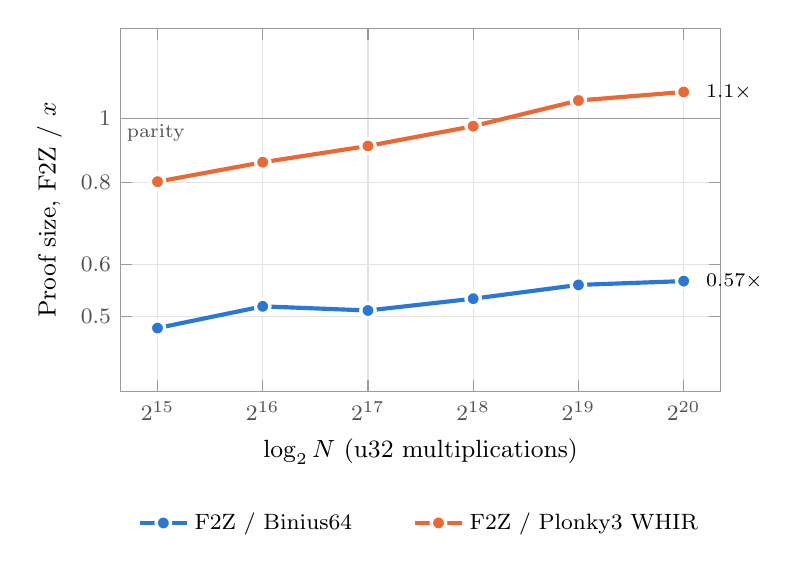
\begin{tikzpicture}
  \begin{axis}[
    width=9.2cm, height=6.2cm,
    xlabel={$\log_2 N$ (u32 multiplications)},
    ylabel={Proof size, F2Z / $x$},
    ymode=log, log basis y=10,
    ytick={0.5,0.6,0.8,1}, yticklabels={0.5,0.6,0.8,1},
    xmin=14.65, xmax=20.35,
    ymin=0.384446, ymax=1.37274,
    xtick={15,16,17,18,19,20}, xticklabels={$2^{15}$,$2^{16}$,$2^{17}$,$2^{18}$,$2^{19}$,$2^{20}$},
    grid=major, grid style={solid, gridgray, line width=0.4pt},
    axis line style={axisgray, line width=0.4pt},
    tick style={axisgray, line width=0.4pt},
    tick label style={font=\footnotesize, text=textmuted},
    label style={font=\small},
    legend style={draw=none, fill=none, font=\footnotesize, cells={anchor=west}, at={(0.5,-0.30)}, anchor=north, legend columns=-1, /tikz/every even column/.append style={column sep=0.7cm}},
    clip=false,
  ]
    % parity: F2Z equal to x
    \addplot[axisgray, line width=0.5pt, forget plot, domain=14.65:20.35, samples=2] {1}
      node[pos=0, anchor=north west, font=\scriptsize, text=textmuted, inner sep=2pt] {parity};
    \addplot[color=sbinius64, line width=1.5pt, mark=*, mark size=2.6pt,
      mark options={fill=sbinius64, draw=surface, line width=1.2pt}]
      coordinates {(15,0.480557) (16,0.518546) (17,0.511063) (18,0.532601) (19,0.558952) (20,0.566493)}
      node[pos=1, anchor=west, xshift=4pt, font=\scriptsize, text=black] {0.57$\times$};
    \addplot[color=splonky3whir, line width=1.5pt, mark=*, mark size=2.6pt,
      mark options={fill=splonky3whir, draw=surface, line width=1.2pt}]
      coordinates {(15,0.802273) (16,0.858754) (17,0.909066) (18,0.974255) (19,1.0659) (20,1.0982)}
      node[pos=1, anchor=west, xshift=4pt, font=\scriptsize, text=black] {1.1$\times$};
    \legend{F2Z / Binius64, F2Z / Plonky3 WHIR}
  \end{axis}
\end{tikzpicture}
\end{document}
